\chapter[Analiza zmogljivosti obla"cne storitve c9]{Analiza zmogljivosti obla"cne storitve Cloud9}

\pagestyle{fancy}
\fancyhf{}
\fancyhead[LE,RO]{\thepage}
\fancyhead[RE,LO]{\leftmark}

\huge "Ziga Kokelj, Tadej Hiti,\\Miha Bizjak, Matej Kristan
\normalsize
\bigskip

\section{Opis problema} \label{8_opis_problema}
\noindent Dana"snje dni se uveljavljajo obla"cne storitve, saj so s stali"s"ca uporabnika najenostavnej"se za uporabo. Na"sa naloga je implementirati prenos datoteke na oz. z obla"cne storitve in breme na obla"cni storitvi, za katero smo si izbrali sortiranje numeri"cnih podatkov.
\noindent Na sliki \ref{8_opis_problema} je grafi"cen prikaz opisanega problema.

\begin{figure}
  \centering
    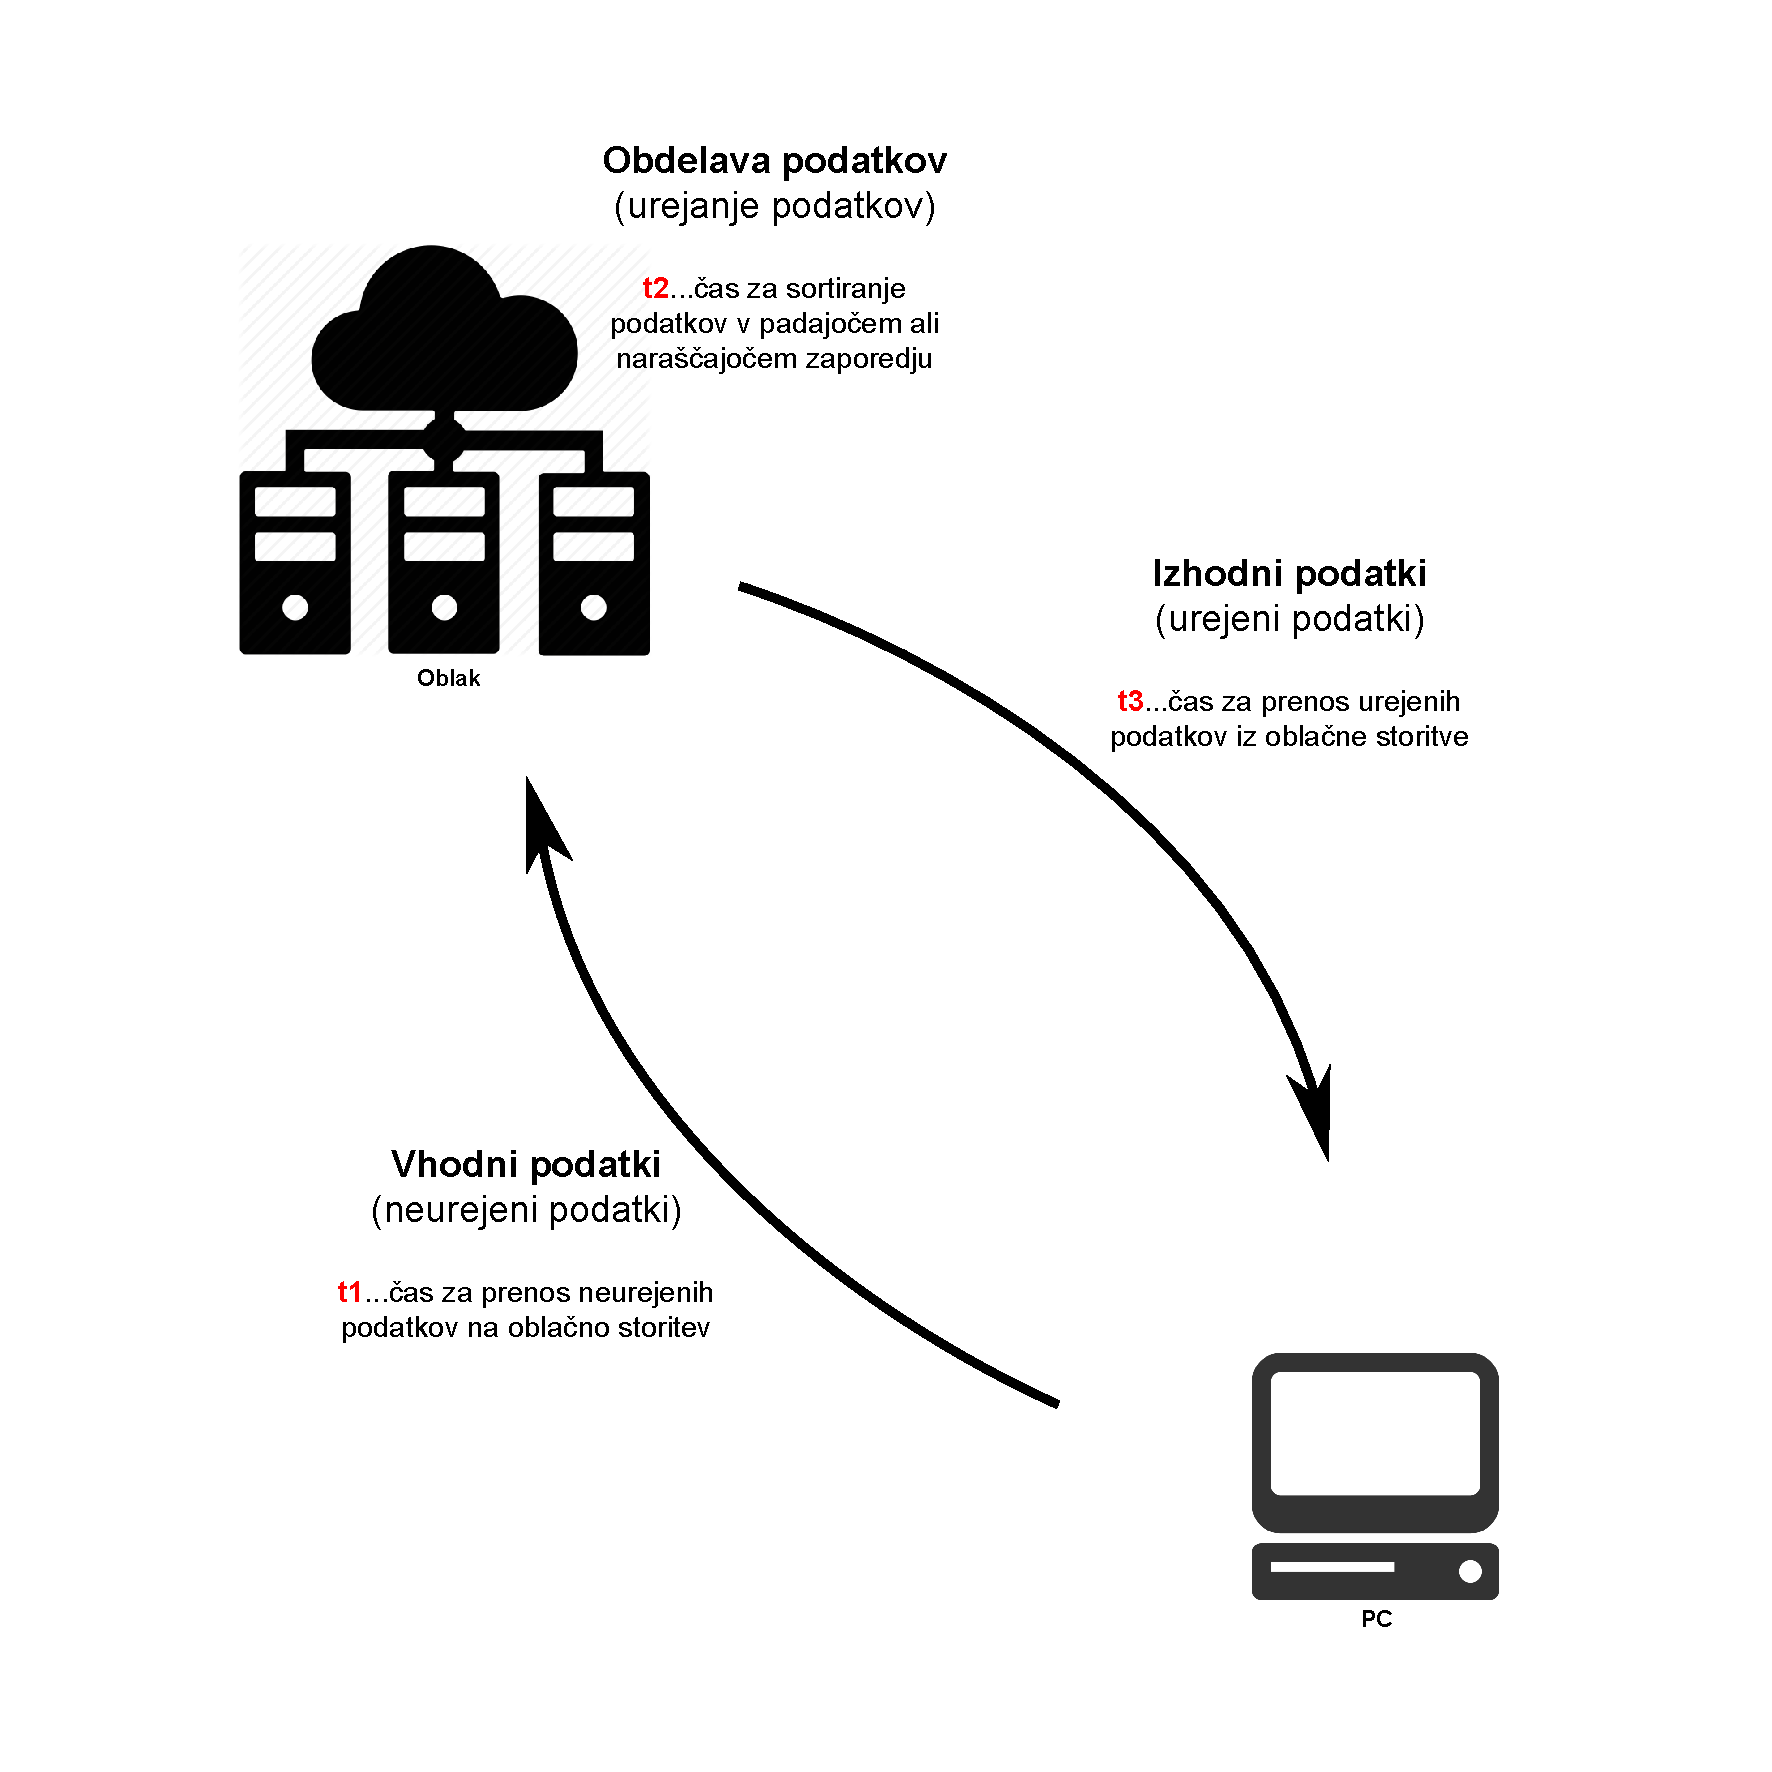
\includegraphics[width=0.74\textwidth]{8_zzrs_opis_problema.pdf}
  \caption{Shema delovanja sistema.}
  \label{8_opis_problema}
\end{figure}


\section{Namen}
Na"se testiranje bo obsegalo merjenje razli"cnih izvajalnih "casov na podlagi katerih bi pri"sli do podatkov o zmogljivosti sistema. Breme sistema bodo razli"cni algoritmi sortiranja podatkov. Namen na"se naloge bo ugotoviti zmogljivost zastonjske ponudbe z vidika razli"cnih metrik zmogljivosti.


\section{Izbira ponudnikov}
Zaradi predhodnih izku"senj z obla"cno storitvijo Cloud9 smo se odlo"cili za njihovo zastonjsko ponudbo. Cloud9 ponuja razvojno okolje in operacijski sistem Ubuntu v katerem lahko pi"semo ali pa izvajamo razli"cne programe.

\subsection{Cloud 9}
Cloud9 je delavno orodje, ki je namenjeno programiranju v brskalniku. Torej vpi"semo URL v brskalnik in "ze imamo vse pripravljeno za pisanje prvega programa. Pri zastonski narocnini nam dajo 512MB primarnega pomnilnika, in 2GB prostora na disku.

\section{Izbira tehnologij}
V tem razdelku so na kratko opisane vse izbrane tehnologije, ki smo jih realizirali sami za na"so analizo.

\subsection{Tehnologija v oblaku}
V obla"cni storitvi smo implementirali stre"znik, ki je napisan v jeziku javascript z uporabo knji"znice Node.js~\cite{8_nodejs}, ki v odvisnosti od URL zahteve posreduje temu primerno datoteko na odjemalca. Stre"znik poskrbi za prena"sanje datotek in zagon sortirnega programa za sortiranje podatkov na stre"zniku.

\subsection{Tehnologija za avtomatizacijo odjemalcev}
Zaradi avtomatskega testiranja smo napisali tudi skripto v programskem jeziku python~\cite{8_python}, ki omogo"ca avtomatsko po"siljanje datoteke in URL zahteve na stre"znik, ter kot odgovor prejme urejeno datoteko z urejenimi podatki. Seveda pa ob tem "se zabele"zimo "cas pred po"siljanjem zahteve in "cas po prejetju urejene datoteke, da dobimo izvajalni "cas celotne procedure. Ker je odjemalcev lahko ve"cje "stevilo, smo ta problem re"sili z nitmi, kjer vsaka nit predstavlja enega odjemalca in po"silja zahteve na stre"znik.

\section{Rezultati meritev}
V tem razdelku so opisani na"cin testiranja na"se  storitve in rezultati meritev.

\subsection{Testiranje I.}
Naklju"cno smo generirali po eno datotek z 10000/15000/20000/25000/30000 integer "stevili, ki jih je nato 1/10/20/30/40/50 odjemalcev po"siljalo na stre"znik. Izmerili smo "case potrebne za prejetje urejene datoteke in pri"sli do povre"cnih "casov. Testiranje je bilo izvedeno okoli popoldneva.  Vse meritve so prikazane na sliki \ref{8_test1} in v tabelah \ref{8_table1}, \ref{8_table2}, \ref{8_table3}, \ref{8_table4}, \ref{8_table5}, kjer je prikazan povre"cen "cas obdelave. Pri datotekah z 25 tiso"c "stevili in 40 do 50 odjemalci je pri"slo do napake 'existing connection was forcibly closed by remote host'. Pri datotekah z 30 tiso"c "stevili in 40 do 50 odjemalci pa nekateri odjemalci po dvo minutnem "cakanju niso dobili odgovora in povezava se prekine. Zakaj in kje pride do napake "se nismo ugotavljali.\\\\

\begin{figure}
  \centering
    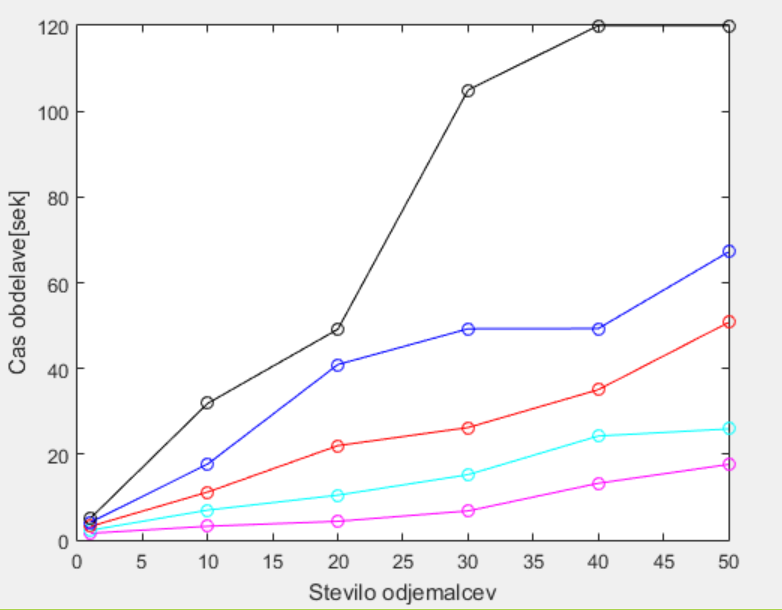
\includegraphics[width=0.65\textwidth]{testiranje_int.png}
  \caption{Graf "casa v odvisnosti od "stevila odjemalcev.}
  \label{8_test1}  
\end{figure}

\begin{figure}
  \centering
  \begin{tabular}{ | c | c | }
    \hline
    "Stevilo odjemalcev & "Cas obdelave[sek]\\ \hline
	1 & 1.57 \\ \hline
    10 & 3.20 \\ \hline
    20 & 4.36 \\ \hline
    30 & 6.78 \\ \hline
    40 & 13.23 \\ \hline
    50 & 17.62 \\ \hline
  \end{tabular}
  \caption{Tabela "casov obdelav datoteke z 10 tiso"c integer "stevili.}
  \label{8_table1}
  \centering
\end{figure}

\begin{figure}
  \centering
  \begin{tabular}{ | c | c | }
    \hline
    "Stevilo odjemalcev & "Cas obdelave[sek]\\ \hline
	1 & 2.27 \\ \hline
    10 & 6.97 \\ \hline
    20 & 10.46 \\ \hline
	30 & 15.23 \\ \hline
    40 & 24.25 \\ \hline
    50 & 25.91 \\ \hline
  \end{tabular}
  \caption{Tabela "casov obdelav datoteke z 15 tiso"c integer "stevili.}
  \label{8_table2}
  \centering
\end{figure}

\begin{figure}
  \centering
  \begin{tabular}{ | c | c | }
    \hline
    "Stevilo odjemalcev & "Cas obdelave[sek]\\ \hline
	1 & 3.18 \\ \hline
    10 & 11.18 \\ \hline
    20 & 22.01 \\ \hline
	30 & 26.23 \\ \hline
    40 & 35.05 \\ \hline
    50 & 50.74 \\ \hline
  \end{tabular}
  \caption{Tabela "casov obdelav datoteke z 20 tiso"c integer "stevili.}
  \label{8_table3}
  \centering
\end{figure}

\begin{figure}
  \centering
  \begin{tabular}{ | c | c | }
    \hline
    "Stevilo odjemalcev & "Cas obdelave[sek]\\ \hline
	1 & 4.16 \\ \hline
    10 & 17.71 \\ \hline
    20 & 40.92 \\ \hline
	30 & 49.26 \\ \hline
    40 & 49.32(napake) \\ \hline
    50 & 67.18(napake) \\ \hline
  \end{tabular}
  \caption{Tabela "casov obdelav datoteke z 25 tiso"c integer "stevili.}
  \label{8_table4}
  \centering
\end{figure}

\begin{figure}
  \centering
  \begin{tabular}{ | c | c | }
    \hline
    "Stevilo odjemalcev & "Cas obdelave[sek]\\ \hline
	1 & 5.09 \\ \hline
    10 & 31.85 \\ \hline
    20 & 49.17 \\ \hline
	30 & 104.93 \\ \hline
    40 & 120+(no answer) \\ \hline
    50 & 120+(no answer) \\ \hline
  \end{tabular}
  \caption{Tabela "casov obdelav datoteke z 30 tiso"c integer "stevili.}
  \label{8_table5}
  \centering
\end{figure}